% Changing book to article will make the footers match on each page,
% rather than alternate every other.
%
% Note that the article class does not have chapters.
\documentclass[letterpaper,10pt,twoside,twocolumn,openany]{book}

% Use babel or polyglossia to automatically redefine macros for terms
% Armor Class, Level, etc...
% Default output is in English; captions are located in lib/dndstring-captions.sty.
% If no captions exist for a language, English will be used.
%1. To load a language with babel:
%	\usepackage[<lang>]{babel}
%2. To load a language with polyglossia:
%	\usepackage{polyglossia}
%	\setdefaultlanguage{<lang>}
\usepackage[english]{babel}
%usepackage[italian]{babel}
% For further options (multilanguage documents, hypenations, language environments...)
% please refer to babel/polyglossia's documentation.

\usepackage[utf8]{inputenc}
\usepackage{hang}
\usepackage{lipsum}
\usepackage{listings}

%packages used for hyperlinking
\usepackage{hyperref}
\hypersetup{
	colorlinks=true,
	linkcolor=blue,
	filecolor=magenta,      
	urlcolor=cyan,
}

\usepackage{dnd}

\lstset{%
  basicstyle=\ttfamily,
  language=[LaTeX]{TeX},
}

\usepackage{eso-pic}
\newcommand\BackgroundPic{%
	\put(0,0){%
		\parbox[b][\paperheight]{\paperwidth}{%
			\vfill
			\centering
			
\includegraphics[width=\paperwidth,height=\paperheight,%
			keepaspectratio]{img/paper.jpg}%
			\vfill
}}}

\title{Milton Manastorm, the Magnificient \\ \vspace{1cm} \\ 
\includegraphics[width=\linewidth]{img/image.jpg}} 	
\author{Antonius Torode}
\date{Latest update: \today}


% Start document
\begin{document}

\AddToShipoutPicture*{\BackgroundPic}
\maketitle
\tableofcontents

% Your content goes here

% Comment this out if you're using the article class.
\chapter{Milton Manastorm Backstory}

Milton Manastorm comes from the Manastorm bloodline and is the twin brother to Millhouse Manastorm. Milton began studying Magic with his twin brother and continued to do so for years. They stuck together for most of their adventures. Of the two, Milton was the practival one who did the majority of work. He learned easier than Millhouse and was able to apply knowledge on a much more realistic level. On the otherwise, Millhouse was similarly just as powerful, but more interested in learning spells such as impending doom, with significantly unpractical cast times. Through their adventures, Milton was always saving his brother from the messes he would get into, secretly enjoying hte chaotic lifestyle they both lived.

Millhouse had a dream as a young boy to become a mage, a wizard. Milton had a similar dream, however he knew his brothers ego would not let them both do the same thing and thus Milton decided to become a sorcerer, allowing his brother to glory in his own self worth (as he saw wizards as the superior beings). As young boys they entered schools of magic, where they were both kicked out. Their mischief (especially when together) was more than the master sorceres and wizards could handle (mentally not physically). The skills and ability to learn magic for the twins was unrivaled. The bond of their bloodline gives them an increased interest and desire to constantly one up each other and enables them to pick up magic very simply.

Together, both the twins traveled all over hunting for rare and priceless artifacts. This was a sort of hobby for them. One day when trying to steal an ancient relic from a mysterious Naaru vessel, the two managed to find themselves split. Millhouse was sent to Arcatraz, a place of imprisonment for dangerous beings the Naaru encountered. He essentially became a stowaway who was in the wrong Naaru vessel at the wrong time. Milton on the other hand, who was similarly on that vessel, tried to escape from the encounter by casting plane shift. Unfortunately the Naaru, who were beings they knew virtually nothing about, caused some interrupting spell which cast Milton onto a far away plane, losing track of his brother. Since this point, they have been on separate paths.

When they were still young, the twins realized how much of a burden and flaw it was to rely on an arcane focus. Unfortunately they were unable to determine a way of not having to have one, but they did solve the flaw in having it be removable. Through a process the twins discovered while trapped (to be used as dinner) in an Orak camp, they found a way to embedd their arcane focus' as part of themselves.  The skin is cut with an Orak knife and pure molten gold is poured into the wound, which was a method the Orak used for tattooing the higher ranking members. Upon killing all members of the camp, they took the needed materials they looted, including the gold, and took it to an acquaintance they had traded a rare artifact to in Aurushire a few months back. This acquaintance was able to safely and very accurately perform this process. 

Milton had two different castings, one on the back of each hand. On the right hand, a hexagon gold cast was poured into his skin, a light red ruby lining with a white crystal in the center sealed in by the gold cast. On the left, a heptagon gold cast, with a dark violet ruby lining, and a black crystal in the center sealed in by the gold cast. On a prior expedition, when the twins were captured to be sacrificed in a village of dark monks, they took note of a balance the monks drew their power from. A balance of light and dark which gave these monks a harmony of power. After freeing themselves and destroying all of the monks, they acquired the most powerful stones from the leaders of the village. The white and black crystals are to represent the different sides of nature and the twins believed if they could harness their power in unison it would give them an enhanced balance of power. Since this time, they have been using the crystals as their arcane focus'.

As it stands, Milton is simply exploring the world, collecting rare and priceless artifacts, learning to increase his power/influence, and finding his brother. 

\chapter{Skills and Features}

\begin{paperbox}[float=!t]{Source of Power}
	The Manastorm bloodline has long been attuned with magic. The source of Milton's power comes from his magical bloodline. Unlike his brother Millhouse, Milton understands this. It does not give him a sense of weakness though. The strong background gives Milton the idea that he is able to do whatever it is he desires.
\end{paperbox}

\section{Class Features}

\subsection{Ability Scores (level 15)}
\stats[
STR = \stat{8},
DEX = \stat{12},
CON = \stat{18},
INT = \stat{16},
WIS = \stat{14},
CHA = \stat{20}
]

\subsection{Traits}
\begin{description}
	\item[Age:] 121
	\item[Alignment:] Chaotic Neutral
	\item[Size:] 2' 7"
	\item[Speed:] 25 ft.
	\item[Darkvision:] Dim light 60 ft as if lit.
	\item[Gnome Cunning:] You have advantage on all
	Intelligence, Wisdom, and Charisma saving throws
	against magic. 
	\item[Languages:] Common, Gnomish
\end{description}

\subsection{Forest Gnome}
\begin{description}
	\item[Natural Illusionist] You know the	minor illusion
	cantrip. Intelligence  is your spellcasting ability for it.
	\item[Speak with Small Beasts:] Through sounds and
	gestures, you can communicate simple ideas with Small
	ar smaller beasts. Forest gnomes love animals and often
	keep squirrels, badgers, rabbits, moles, woodpeckers,
	and other creatures as beloved pets.
\end{description}

\subsection{Hit Points}

\begin{description}[font=\normalfont\textbf,noitemsep,topsep=1ex,leftmargin=1em]
	\item[Hit Dice:] 1d6 per level
	\item[Hit Points at First Level:] 6 + constitution modifier
	\item[Hit Points at Higher levels:] 1d6 (or 4) + constitution modifier per level 
\end{description}

\subsection{Proficiencies}

\begin{description}[font=\normalfont\textbf,noitemsep,topsep=1ex,leftmargin=1em]
	\item[Armor:] None
	\item[Weapons:] Daggers, darts, slings, quarterstaff's, light crossbows 
	\item[Tools:] None 
\end{description}

\begin{description}[font=\normalfont\textbf,noitemsep,topsep=1ex,leftmargin=1em]
	\item[Saving Throws:] Constitution, Charisma
	\item[Skills:] Insight, Deception
\end{description}

\subsection{Equipment}

\begin{description}
	\item[Arcane Focus:] See backstory
	\item[Two Daggers:] Normal daggers, very sharp.
	\item[Stone of Good Luck:] While this polished agate is on your person, you gain a +1 bonus to Ability Checks and saving throws.
	\item[Gauntlets of Ogre Power:] Your Strength score is 19 while you wear these gauntlets. They have no effect on you if your Strength is already 19 or higher without them.
	\item[Cloak of Displacement:] While you wear this cloak, it projects an Illusion that makes you appear to be standing in a place near your actual location, causing any creature to have disadvantage on Attack rolls against you. If you take damage, the property ceases to function until the start of your next turn. This property is suppressed while you are Incapacitated, Restrained, or otherwise unable to move.
	\item[Bracers of Defense:] While wearing these bracers, you gain a +2 bonus to AC if you are wearing no armor and using no shield.
	\item[Quarterstaff:] An wooden staff with an embedded star ruby in the end. The wood is enchanted to be as hard as steel.
\end{description}

\subsection{Cantrips}

\begin{description}
	\item[Natural Illusionist:] \hyperlink{Minor Illusion}{Minor Illusion}
	\item[Level 1:] \hyperlink{Fire Bolt}{Fire Bolt}, \hyperlink{Prestidigitation}{Prestidigitation}, \hyperlink{Light}{Light}, \hyperlink{Mage Hand}{Mage Hand}
	\item[Level 4:] \hyperlink{True Strike}{True Strike}
	\item[Level 10:] \hyperlink{Shocking Grasp}{Shocking Grasp}
\end{description}

\subsection{Spells}

\begin{description}
	\item[Level 1:] \hyperlink{Magic Missile (1)}{Magic Missile (1)}, \hyperlink{Mage Armor (1)}{Mage Armor (1)}
	\item[Level 2:] \hyperlink{Shield (1)}{Shield (1)}
	\item[Level 3:] \hyperlink{Scorching Ray (2)}{Scorching Ray (2)}	 
	\item[Level 4:] \hyperlink{Mirror Image (2)}{Mirror Image (2)}
	\item[Level 5:] \hyperlink{Lightning Bolt (3)}{Lightning Bolt (3)}
	\item[Level 6:] \hyperlink{Blink (3)}{Blink (3)}
	\item[Level 7:] \hyperlink{Fireball (3)}{Fireball (3)}
	\item[Level 8:] \hyperlink{Greater Invisibility (4)}{Greater Invisibility (4)}
	\item[Level 9:] \hyperlink{Confusion (4)}{Confusion (4)}
	\item[Level 10:] \hyperlink{Hold Monster (5)}{Hold Monster (5)}
	\item[Level 11:] \hyperlink{Disintegrate (6)}{Disintegrate (6)}
	\item[Level 12:]
	\item[Level 13:] \hyperlink{Finger of Death (7)}{Finger of Death (7)}
	\item[Level 14:] 
	\item[Level 15:] \hyperlink{Dominate Monster (8)}{Dominate Monster (8)}
\end{description}

\subsection{Spellcasting Ability}

\begin{description}
	\item[Spell save DC:] 8+proficiency bonus + charisma modifier
	\item[Spell attack modifier:] proficiency bonus + charisma modifier
\end{description}

\subsection{Flexible Casting}

\begin{description}
	\item[Creating Spell Slots: ] You can transform unexpended sorcery points into one spell slot as a bonus action on your turn.
\begin{dndtable}
	\textbf{Spell Slot Level}  & \textbf{Sorcery Point Cost} \\
	1st  & 2 \\
	2nd & 3 \\
	3rd & 5 \\
	4th & 6 \\
	5th & 7
\end{dndtable}
	\item[Converting a Spell Slot to Sorcery Points:] As a bonus action on your turn, you can expend one spell slot and gain a number of sorcery points equal to the slot's level.
\end{description}

\subsection{Metamagic}

\begin{description}
	\item[Quickened Spall:] When you cast a spell that has a casting time of 1 action, you can spend 2 sorcery points to change the casting time to 1 bonus action for this casting.
	\item[Empowered Spell:] When you roll damage for a spell, you can spend 1
	sorcery point to re-roll a number of the damage dice up to your Charisma modifier (minimum of one). You must use the new rolls. You can use Empowered Spell even if you have already used a different Metamagic option during the casting of the spell.
	\item[Heightened Spell:] When you cast a spell that forces a creature to make a saving throw to resist its effects, you can spend 3 sorcery points to give one target of the spell disadvantage on its first saving throw made against the spell.
\end{description}

\subsection{Phoenix Sorcery}

\begin{description}
	\item[Ignite:] As an action, you can magically ignite a flammable object you touch with your hand. 
	\item[Mantle of Flame:] As a bonus action, you magically wreathe yourself in swirling fire. For 1 minute, you gain the following benefits:
	
	\begin{enumerate}
		\item You shed bright light in a 30-foot radius and dim light for an additional 30 feet.
		\item Any creature takes fire damage equal to your Charisma modifier if it hits you with a melee attack from within 5 feet of you or if it touches you.
		\item Whenever you roll fire damage on your turn, the roll gains a bonus to equal to your Charisma modifier. 
	\end{enumerate}
	
	Once you use this feature, you can't use it again until you finish a long rest. 
	\item[Phoenix Spark:]  if you are reduced to 0 hit points, you can use your reaction instead be reduced to 1 hit point, and each creature within 10 feet of you takes fire damage equal to half your sorcerer level + your Charisma modifier.
	
	If you use this feature while under the effects of your Mantle of Flame, this feature instead deals fire damage equal to your sorcerer level + double your Charisma modifier, and your Mantle of Flame immediately ends. Once you use this feature, you can't use it again until you finish a long rest. 
	\item[Nourishing Fire:] When you expend a spell slot to cast a spell that includes a fire damage roll, you regain hit points equal to the slot's level + your Charisma modifier. 
\end{description}

\subsection{Sage}
\begin{description}[font=\normalfont\textbf,noitemsep,topsep=1ex,leftmargin=1em]
	\item[Skill Proficiencies:] Arcana, History
	\item[Languages:] Draconic, Celestial
	\item[Equipment:] A bottle of black ink, a quill, a small knife, a letter from a dead colleague posing a question you have not yet been able to answer, a set of common clothes, and a belt pouch containing 10 gp
	\item[Feature - Researcher:] When you attempt to learn or recall a piece of lore, if you do not know that information, you often know where and from whom you can obtain it. Usually, this information comes from a library, scriptorium, university, or a sage or other learned person or creature. Your DM might rule that the knowledge you seek is secreted away in an almost inaccessible place, or that it simply cannot be found. Unearthing the deepest secrets of the multiverse can require an adventure or even a whole campaign. 
\end{description}

\subsection{Personality}

\begin{description}
	\item[Trait:] I use polysyllabic words that convey the impression of great erudition.
\end{description}

\subsection{Quotes}


\begin{description}
	\item[] "<adjective>"? I don't care who you are, friend: nobody refers to the mighty Milton Manastorm as "<adjective>"!
	\item[] I have no idea what goes on here, but I will gladly join your fight against this impudent imbecile! Prepare to defend yourself, cretin!
	\item[] I just need to get some things ready first. You guys go ahead and get started. I need to summon up some water...
	\item[] Aaalllriiiight!! Who ordered up an extra large can of whoop-ass?
	\item[] I'm gonna light you up, sweet cheeks!
	\item[] I didn't even break a sweat on that one
	\item[] You guys feel free to jump in anytime.
	\item[] Heal me! For the love of all that's holy, heal me! I'm dying!!
	\item[] It's time for a tactical retreat!
	\item[] Prison taught me one very important lesson, well, two if you count how to hold your soap, but yes! SURVIVAL!
	\item[] Now... witness the full power of Milton Manastorm!
	\item[] If you have any excess priceless artifacts that were lost in time, I'm making a collection.
	\item[] Have you ever been hit in the face by a worm made out of rocks? It feels like what it sounds like.
	\item[] You will all be my slaves! Er, I mean, hi!
	\item[] When do we destroy the world? Soon? I hope it's soon.
	\item[] You wouldn't happen to have access to any N.U.K.U.L.A.R. weapons, would you?
	\item[] Let's just say I have friends in high places...
	\item[] I've killed cockroaches bigger than that!
	\item[] Sometimes I talk to myself because I like dealing with a... better class of people.
	\item[] Someone told me I was arrogant once. I'm not arrogant, I'm just better.
	\item[] That's okay, nobody is perfect. Wow, that must mean I'm nobody.
	\item[] You cant spell awesome with me.
	
\end{description}










\onecolumn
\section{Sorcerer Leveling Table}
\begin{center}
	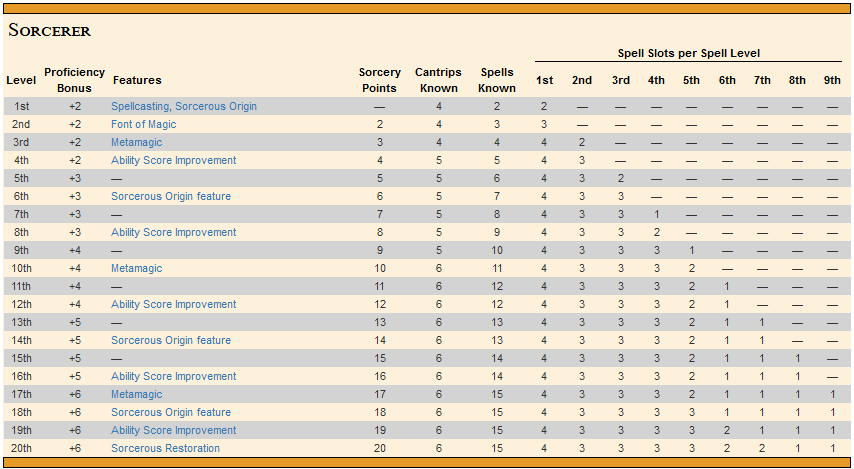
\includegraphics[width=\linewidth]{img/SpellSlotTable.png}
\end{center}

\twocolumn

\section{Spells}

\subsection{Fire Bolt} \hypertarget{Fire Bolt}{}
\begin{hangingpar}
	\textit{Evocation cantrip}
\end{hangingpar}

\begin{description}
	\item[Casting Time:] 1 action
	\item[Range:] 120 feet
	\item[Components:] V,S
	\item[Duration:] Instantaneous
\end{description}

You hurl a mote of fire at a creature or object within range. Make a ranged spell attack against the target. On a hit, the target takes 1d10 fire damage. A flammable object hit by this spell ignites if it isn't being worn or carried.
This spell's damage increases by 1d10 when you reach 5th level (2d10), 11th level (3d10), and 17th level (4d10).



\subsection{Prestidigitation} \hypertarget{Prestidigitation}{}
\begin{hangingpar}
	\textit{Transmutation cantrip}
\end{hangingpar}

\begin{description}
	\item[Casting Time:] 1 action 
	\item[Range:] 10 feet 
	\item[Components:] V, S 
	\item[Duration:] Up to 1 hour 
\end{description}

This spell is a minor magical trick that novice spellcasters use for practice. You create one of the following magical effects within range:

\begin{enumerate}
	\item You create an instantaneous, harmless sensory effect, such as a shower of sparks, a puff of wind, faint musical notes, or an odd odor.
	\item You instantaneously light or snuff out a candle, a torch, or a small campfire.
	\item You instantaneously clean or soil an object no larger than 1 cubic foot.
	\item You chill, warm, or flavor up to 1 cubic foot of nonliving material for 1 hour.
	\item You make a color, a small mark, or a symbol appear on an object or a surface for 1 hour.
	\item You create a nonmagical trinket or an illusory image that can fit in your hand and that lasts until the end of your next turn.
\end{enumerate}

If you cast this spell multiple times, you can have up to three of its non-instantaneous effects active at a time, and you can dismiss such an effect as an action. 

\subsection{Minor Illusion} \hypertarget{Minor Illusiont}{}
\begin{hangingpar}
	\textit{Illusion cantrip}
\end{hangingpar}

\begin{description}
	\item[Casting Time:] 1 action 
	\item[Range:] 30 feet 
	\item[Components:] S, M (a bit of fleece)
	\item[Duration:] 1 minute 
\end{description}

You create a sound or an image of an object within range that lasts for the duration. The illusion also ends if you dismiss it as an action or cast this spell again.

If you create a sound, its volume can range from a whisper to a scream. It can be your voice, someone else's voice, a lion's roar, a beating of drums, or any other sound you choose. The sound continues unabated throughout the duration, or you can make discrete sounds at different times before the spell ends.

If you create an image of an object--such as a chair, muddy footprints, or a small chest--it must be no larger than a 5-foot cube. The image can't create sound, light, smell, or any other sensory effect. Physical interaction with the image reveals it to be an illusion, because things can pass through it.

If a creature uses its action to examine the sound or image, the creature can determine that it is an illusion with a successful Intelligence (Investigation) check against your spell save DC. If a creature discerns the illusion for what it is, the illusion becomes faint to the creature. 

\subsection{Light} \hypertarget{Light}{}
\begin{hangingpar}
	\textit{Evocation cantrip}
\end{hangingpar}

\begin{description}
	\item[Casting Time:] 1 action 
	\item[Range:] Touch 
	\item[Components:] V, M (a firefly or phosphorescent moss) 
	\item[Duration:] 1 hour 
\end{description}

You touch one object that is no larger than 10 feet in any dimension. Until the spell ends, the object sheds bright light in a 20-foot radius and dim light for an additional 20 feet. The light can be colored as you like. Completely covering the object with something opaque blocks the light. The spell ends if you cast it again or dismiss it as an action.

If you target an object held or worn by a hostile creature, that creature must succeed on a Dexterity saving throw to avoid the spell.

\subsection{Mage Hand} \hypertarget{Mage Hand}{}
\begin{hangingpar}
	\textit{Conjuration cantrip}
\end{hangingpar}

\begin{description}
	\item[Casting Time:]  1 action 
	\item[Range:] 30 feet 
	\item[Components:] V, S 
	\item[Duration:] 1 minute A spectral, floating hand appears at a point you choose within range. The hand lasts for the duration or until you dismiss it as an action. The hand vanishes if it is ever more than 30 feet away from you or if you cast this spell again. 
\end{description}

You can use your action to control the hand. You can use the hand to manipulate an object, open an unlocked door or container, stow or retrieve an item from an open container, or pour the contents out of a vial. You can move the hand up to 30 feet each time you use it.

The hand can't attack, activate magic items, or carry more than 10 pounds. 

\subsection{True Strike} \hypertarget{True Strike}{}
\begin{hangingpar}
	\textit{Divination cantrip}
\end{hangingpar}

\begin{description}
	\item[Casting Time:] 1 action 
	\item[Range:] 30 feet 
	\item[Components:] S 
	\item[Duration:] Concentration, up to 1 round 
\end{description}

You extend your hand and point a finger at a target in range. Your magic grants you a brief insight into the target's defenses. On your next turn, you gain advantage on your first attack roll against the target, provided that this spell hasn't ended.

\subsection{Shocking Grasp} \hypertarget{Shocking Grasp}{}
\begin{hangingpar}
	\textit{Evocation cantrip}
\end{hangingpar}

\begin{description}
	\item[Casting Time:] 1 action 
	\item[Range:] Touch 
	\item[Components:] V, S
	\item[Duration:] Instantaneous
\end{description}

Lightning springs from your hand to deliver a shock to a creature you try to touch. Make a melee spell attack against the target. You have advantage on the attack roll if the target is wearing armor made of metal. On a hit, the target takes 1d8 lightning damage, and it can't take reactions until the start of its next turn.

The spell's damage increases by 1d8 when you reach 5th level (2d8), 11th level (3d8), and 17th level (4d8). 

\subsection{Magic Missile} \hypertarget{Magic Missile}{}
\begin{hangingpar}
	\textit{1st-level evocation}
\end{hangingpar}

\begin{description}
	\item[Casting Time:] 1 action 
	\item[Range:] 120 feet
	\item[Components:] V, S 
	\item[Duration:] Instantaneous 
\end{description}

You create three glowing darts of magical force. Each dart hits a creature of your choice that you can see within range. A dart deals 1d4 + 1 force damage to its target. The darts all strike simultaneously, and you can direct them to hit one creature or several. 

\begin{description}
	\item[At Higher Levels] When you cast this spell using a spell slot of 2nd level or higher, the spell creates one more dart for each slot level above 1st.
\end{description}

\subsection{Mage Armor} \hypertarget{Mage Armor}{}
\begin{hangingpar}
	\textit{1st-level abjuration}
\end{hangingpar}

\begin{description}
	\item[Casting Time:] 1 action 
	\item[Range:] Touch 
	\item[Components:] V, S, M (a piece of cured leather)
	\item[Duration:] 8 hours 
\end{description}

You touch a willing creature who isn't wearing armor, and a protective magical force surrounds it until the spell ends. The target's base AC becomes 13 + its Dexterity modifier. The spell ends if the target dons armor or if you dismiss the spell as an action. 

\subsection{Shield} \hypertarget{Shield}{}
\begin{hangingpar}
	\textit{1st-level abjuration}
\end{hangingpar}

\begin{description}
	\item[Casting Time:]  1 reaction, which you take when you are hit by an attack or targeted by the magic missile spell 
	\item[Range:] Self 
	\item[Components:] V, S 
	\item[Duration:] 1 round 
\end{description}

An invisible barrier of magical force appears and protects you. Until the start of your next turn, you have a +5 bonus to AC, including against the triggering attack, and you take no damage from magic missile. 

\subsection{Scorching Ray} \hypertarget{Scorching Ray}{}
\begin{hangingpar}
	\textit{2nd-level evocation}
\end{hangingpar}

\begin{description}
	\item[Casting Time:] 1 action
	\item[Range:] 120 feet 
	\item[Components:] V, S
	\item[Duration:] Instantaneous
\end{description}

You create three rays of fire and hurl them at targets within range. You can hurl them at one target or several.

Make a ranged spell attack for each ray. On a hit, the target takes 2d6 fire damage. 

\begin{description}
	\item[At Higher Levels] When you cast this spell using a spell slot of 3rd level or higher, you create one additional ray for each slot level above 2nd. 
\end{description}

\subsection{Mirror Image} \hypertarget{Mirror Image}{}
\begin{hangingpar}
	\textit{2nd-level illusion}
\end{hangingpar}

\begin{description}
	\item[Casting Time:] 1 action
	\item[Range:] Self 
	\item[Components:] V, S
	\item[Duration:] 1 minute
\end{description}

Three illusory duplicates of yourself appear in your space. Until the spell ends, the duplicates move with you and mimic your actions, shifting position so it's impossible to track which image is real. You can use your action to dismiss the illusory duplicates.

Each time a creature targets you with an attack during the spell's duration, roll a d20 to determine whether the attack instead targets one of your duplicates.

If you have three duplicates, you must roll a 6 or higher to change the attack's target to a duplicate. With two duplicates, you must roll an 8 or higher. With one duplicate, you must roll an 11 or higher.

A duplicate's AC equals 10 + your Dexterity modifier. If an attack hits a duplicate, the duplicate is destroyed. A duplicate can be destroyed only by an attack that hits it. It ignores all other damage and effects. The spell ends when all three duplicates are destroyed.

A creature is unaffected by this spell if it can't see, if it relies on senses other than sight, such as blindsight, or if it can perceive illusions as false, as with truesight. 

\subsection{Lightning Bolt} \hypertarget{Lightning Bolt}{}
\begin{hangingpar}
	\textit{3rd-level evocation}
\end{hangingpar}

\begin{description}
	\item[Casting Time:] 1 action
	\item[Range:] Self (100-foot line)
	\item[Components:] V, S, M (a bit of fur and a rod of amber, crystal, or glass) 
	\item[Duration:] Instantaneous
\end{description}

A stroke of lightning forming a line 100 feet long and 5 feet wide blasts out from you in a direction you choose. Each creature in the line must make a Dexterity saving throw. A creature takes 8d6 lightning damage on a failed save, or half as much damage on a successful one.

The lightning ignites flammable objects in the area that aren't being worn or carried. 

\begin{description}
	\item[At Higher Levels] When you cast this spell using a spell slot of 4th level or higher, the damage increases by 1d6 for each slot level above 3rd.
\end{description}

\subsection{Blink} \hypertarget{Blink}{}
\begin{hangingpar}
	\textit{3rd-level transmutation}
\end{hangingpar}

\begin{description}
	\item[Casting Time:] 1 action
	\item[Range:] Self 
	\item[Components:] V, S
	\item[Duration:] 1 minute
\end{description}

Roll a d20 at the end of each of your turns for the duration of the spell. On a roll of 11 or higher, you vanish from your current plane of existence and appear in the Ethereal Plane (the spell fails and the casting is wasted if you were already on that plane). At the start of your next turn, and when the spell ends if you are on the Ethereal Plane, you return to an unoccupied space of your choice that you can see within 10 feet of the space you vanished from. If no unoccupied space is available within that range, you appear in the nearest unoccupied space (chosen at random if more than one space is equally near). You can dismiss this spell as an action.

While on the Ethereal Plane, you can see and hear the plane you originated from, which is cast in shades of gray, and you can't see anything there more than 60 feet away. You can only affect and be affected by other creatures on the Ethereal Plane. Creatures that aren't there can't perceive you or interact with you, unless they have the ability to do so. 

\subsection{Fireball} \hypertarget{Fireball}{}
\begin{hangingpar}
	\textit{3rd-level evocation}
\end{hangingpar}

\begin{description}
	\item[Casting Time:] 1 action
	\item[Range:] 150 feet 
	\item[Components:] V, S, M (a tiny ball of bat guano and sulfur) 
	\item[Duration:] Instantaneous 
\end{description}

A bright streak flashes from your pointing finger to a point you choose within range and then blossoms with a low roar into an explosion of flame. Each creature in a 20-foot-radius sphere centered on that point must make a Dexterity saving throw. A target takes 8d6 fire damage on a failed save, or half as much damage on a successful one.

The fire spreads around corners. It ignites flammable objects in the area that aren't being worn or carried. 

\begin{description}
	\item[At Higher Levels] When you cast this spell using a spell slot of 4th level or higher, the damage increases by 1d6 for each slot level above 3rd. 
\end{description}

\subsection{Greater Invisibility} \hypertarget{Greater Invisibility}{}
\begin{hangingpar}
	\textit{4th-level illusion}
\end{hangingpar}

\begin{description}
	\item[Casting Time:] 1 action
	\item[Range:] Touch 
	\item[Components:] V, S
	\item[Duration:] Concentration, up to 1 minute
\end{description}

You or a creature you touch becomes invisible until the spell ends. Anything the target is wearing or carrying is invisible as long as it is on the target's person. 

\subsection{Confusion} \hypertarget{Confusion}{}
\begin{hangingpar}
	\textit{4th-level enchantment}
\end{hangingpar}

\begin{description}
	\item[Casting Time:] 1 action
	\item[Range:] 90 feet 
	\item[Components:] V, S, M (three nut shells) 
	\item[Duration:] Concentration, up to 1 minute
\end{description}

This spell assaults and twists creatures' minds, spawning delusions and provoking uncontrolled action. Each creature in a 10-foot-radius sphere centered on a point you choose within range must succeed on a Wisdom saving throw when you cast this spell or be affected by it.

An affected target can't take reactions and must roll a d10 at the start of each of its turns to determine its behavior for that turn. 

\begin{description}
	\item[1.] The creature uses all its movement to move in a random direction. To determine the direction, roll a d8 and assign a direction to each die face. The creature doesn't take an action this turn.
	\item[2-6.] The creature doesn't move or take actions this turn.
	\item[7-8.] The creature uses its action to make a melee attack against a randomly determined creature within its reach. If there is no creature within its reach, the creature does nothing this turn.
	\item[9-10.] The creature can act and move normally.
\end{description}

At the end of each of its turns, an affected target can make a Wisdom saving throw. If it succeeds, this effect ends for that target. 

\begin{description}
	\item[At Higher Levels] When you cast this spell using a spell slot of 5th level or higher, the radius of the sphere increases by 5 feet for each slot level above 4th.
\end{description}

\subsection{Hold Monster} \hypertarget{Hold Monster}{}
\begin{hangingpar}
	\textit{5th-level enchantment}
\end{hangingpar}
\begin{description}
	\item[Casting Time:] 1 action
	\item[Range:] 90 feet
	\item[Components:] V, S, M (a small, straight piece of iron) 
	\item[Duration:] Concentration, up to 1 minute 
\end{description}

Choose a creature that you can see within range. The target must succeed on a Wisdom saving throw or be paralyzed for the duration. This spell has no effect on undead. At the end of each of its turns, the target can make another Wisdom saving throw. On a success, the spell ends on the target.

\begin{description}
	\item[At Higher Levels] When you cast this spell using a spell slot of 6th level or higher, you can target one additional creature for each slot level above 5th. The creatures must be within 30 feet of each other when you target them.
\end{description}

\subsection{Disintegrate} \hypertarget{Disintegrate}{}
\begin{hangingpar}
	\textit{6th-level transmutation}
\end{hangingpar}
\begin{description}
	\item[Casting Time:] 1 action
	\item[Range:] 60 feet 
	\item[Components:] V, S, M (a lodestone and a pinch of dust) 
	\item[Duration:] Instantaneous 
\end{description}

A thin green ray springs from your pointing finger to a target that you can see within range. The target can be a creature, an object, or a creation of magical force, such as the wall created by wall of force.

A creature targeted by this spell must make a Dexterity saving throw. On a failed save, the target takes 10d6 + 40 force damage. If this damage reduces the target to 0 hit points, it is disintegrated.

A disintegrated creature and everything it is wearing and carrying, except magic items, are reduced to a pile of fine gray dust. The creature can be restored to life only by means of a true resurrection or a wish spell.

This spell automatically disintegrates a Large or smaller nonmagical object or a creation of magical force. If the target is a Huge or larger object or creation of force, this spell disintegrates a 10-foot- cube portion of it. A magic item is unaffected by this spell.

\begin{description}
	\item[At Higher Levels] When you cast this spell using a spell slot of 7th level or higher, the damage increases by 3d6 for each slot level above 6th
\end{description}

\subsection{Finger of Death} \hypertarget{Finger of Death}{}
\begin{hangingpar}
	\textit{7th-level necromancy}
\end{hangingpar}
\begin{description}
	\item[Casting Time:] 1 action
	\item[Range:] 60 feet
	\item[Components:] V, S
	\item[Duration:] Instantaneous 
\end{description}

You send negative energy coursing through a creature that you can see within range, causing it searing pain. The target must make a Constitution saving throw. It takes 7d8 + 30 necrotic damage on a failed save, or half as much damage on a successful one.

A humanoid killed by this spell rises at the start of your next turn as a zombie that is permanently under your command, following your verbal orders to the best of its ability.

\subsection{Dominate Monster} \hypertarget{Dominate Monster}{}
\begin{hangingpar}
	\textit{8th-level enchantment}
\end{hangingpar}
\begin{description}
	\item[Casting Time:] 1 action
	\item[Range:] 60 feet 
	\item[Components:] V, S 
	\item[Duration:] Concentration, up to 1 hour 
\end{description}

You attempt to beguile a creature that you can see within range. It must succeed on a Wisdom saving throw or be charmed by you for the duration. If you or creatures that are friendly to you are fighting it, it has advantage on the saving throw.

While the creature is charmed, you have a telepathic link with it as long as the two of you are on the same plane of existence. You can use this telepathic link to issue commands to the creature while you are conscious (no action required), which it does its best to obey. You can specify a simple and general course of action, such as "Attack that creature," "Run over there," or "Fetch that object." If the creature completes the order and doesn't receive further direction from you, it defends and preserves itself to the best of its ability.

You can use your action to take total and precise control of the target. Until the end of your next turn, the creature takes only the actions you choose, and doesn't do anything that you don't allow it to do. During this time, you can also cause the creature to use a reaction, but this requires you to use your own reaction as well.

Each time the target takes damage, it makes a new Wisdom saving throw against the spell. If the saving throw succeeds, the spell ends. 

\begin{description}
	\item[At Higher Levels] When you cast this spell with a 9th-level spell slot, the duration is concentration, up to 8 hours.
\end{description}

% End document
\end{document}
